\documentclass[10pt]{exam}
\usepackage[hon]{template-for-exam}
\usepackage{my-tikz-clipart}
\usepackage{multicol}
\usepackage{graphicx}
\graphicspath{{./FBDs}}


\title{Free-Body Diagrams \& Single-Body Force Problems}
\author{Rohrbach}
\date{\today}

\begin{document}
\maketitle

\begin{questions}

  \question
  For each of the sketches below, identify all the forces applied on all objects and draw a free body diagram.  Then come up with an expression for the net force.


  \begin{multicols}{2}
    \begin{parts}
      \part 
        Lamp hanging from a chain

        \begin{center}
          \begin{tikzpicture}
            \clip (-3,-3) rectangle (3,3);
            \node[rotate=180,opacity=0.5] at (0,0) (bulb) {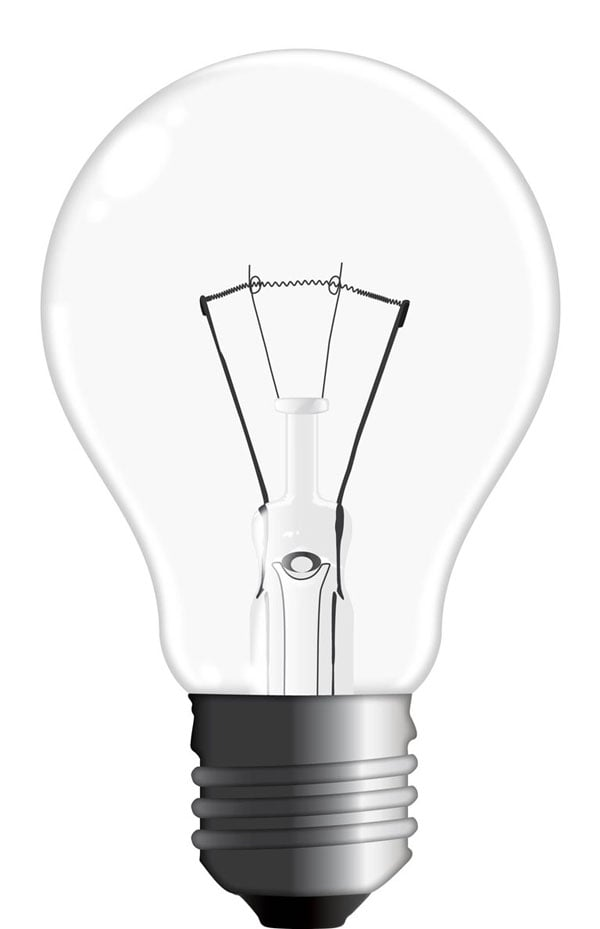
\includegraphics[width=1cm]{bulb.jpg}};
            \filldraw[pattern=north east lines,pattern color=gray,draw=gray] 
              (-.045,0.8) -- ++(.07,0) -- ++(0,3) -- ++(-.1,0) -- cycle;

            


          \end{tikzpicture}
        \end{center}

        
        

      \part 
        A car moving at a constant speed.

        \begin{center}
            \begin{tikzpicture}
              \clip (-3,-3) rectangle (3,3);
              \begin{scope}[shift={(-1.5,0)},scale=0.5]
                 \draw[gray,rounded corners]
                    (0,0) -- (0,1) -- (4.5,1) -- 
                    (5.5,.6) -- (5.5,0) -- cycle;
                  \draw[gray] 
                    (1,1) -- (1.5,1.75) -- (3,1.75) -- 
                    (4,1) -- cycle;
                  \draw[gray, fill=gray!20, thick] 
                    (1,0) circle (.5);
                  \draw[gray, fill=gray!20, thick] 
                    (4.5,0) circle (.5);
              \end{scope}
              \draw[gray] (-3,-0.25) -- ++(6,0);
            \end{tikzpicture}
          \end{center}

      
      \part 
        A car accelerating

           \begin{center}
            \begin{tikzpicture}
              \clip (-3,-3) rectangle (3,3);
              \begin{scope}[shift={(-1.5,0)},scale=0.5]
                 \draw[gray,rounded corners]
                    (0,0) -- (0,1) -- (4.5,1) -- 
                    (5.5,.6) -- (5.5,0) -- cycle;
                  \draw[gray] 
                    (1,1) -- (1.5,1.75) -- (3,1.75) -- 
                    (4,1) -- cycle;
                  \draw[gray, fill=gray!20, thick] 
                    (1,0) circle (.5);
                  \draw[gray, fill=gray!20, thick] 
                    (4.5,0) circle (.5);
              \end{scope}
              \draw[gray] (-3,-0.25) -- ++(6,0);
            \end{tikzpicture}
          \end{center}

            

      \columnbreak

      \part 
        A box being pushed forward on the ground (constant speed)

        \begin{center}
            \begin{tikzpicture}
              \clip (-3,-3) rectangle (3,3);
              \begin{scope}
                \draw[gray] (-3,0) -- (3,0);
                \draw[gray, rounded corners] 
                  (-0.5,0) rectangle (0.5,1);
              \end{scope}
              \begin{scope}[draw=gray,rounded corners,shift={(-0.8,0)}]
                \draw (0.1,1.2) circle (0.2);
                \coordinate (waste) at (-.2,.5);
                \coordinate (neck) at (0.1,1);
                \draw (waste) -- (neck);
                \draw (-.7,0.4) -- ++(0.3,-0.15) -- (waste);
                \draw (0,0) -- ++(0.15,0.2) -- (waste);
                \draw (neck) -- +(0,-.3) -- +(.2,-.3);
                \draw (neck) -- +(-.3,-.3) -- +(.2,-.4);
              \end{scope}
            \end{tikzpicture}
          \end{center}

      \part 
        A skydiver before opening her parachute

        \begin{center}
            \begin{tikzpicture}
              \clip (-3,-3) rectangle (3,3);
              \begin{scope}[draw=gray,scale=1.5]
                \draw (0,0) circle (0.2);
                \coordinate (neck) at (-0.2,0);
                \path (neck) ++(-160:0.7) coordinate (waste);
                \draw (waste) -- (neck);
                \draw[rounded corners] (neck) -- ++(-0.1,-.4) -- ++(.4,.1);
                \draw[rounded corners] (neck) -- ++(0,.4) -- ++(.4,-.1);
                \draw (waste) -- ++(-0.5,0);
                \draw (waste) -- ++(-0.3,-0.4);

                \begin{scope}
                  \fill[black!40,rounded corners=3px] (neck) -- ++(-160:0.4) -- ++(-250:0.15) -- ++(20:0.4) -- cycle;
                \end{scope}

              \end{scope}
            \end{tikzpicture}
          \end{center}
        

      \part 
        Object sliding down an inclined plane.

          \begin{center}
            \begin{tikzpicture}
              \clip (-3,-3) rectangle (3,3);
              \begin{scope}[rotate=-30]
                \draw[gray] (-2,0) -- (2,0);
                \draw[gray, rounded corners] 
                  (-0.5,0) rectangle (0.5,1);
              \end{scope}
            \end{tikzpicture}
          \end{center}

      
    \end{parts}
    
  \end{multicols}
  
\question
  Neal is stealing a refrigerator from the bank.  The mass of the refrigerator is \SI{173}{\kilo\gram} and its kinetic friction has a magnitude of \SI{254}{\newton}.  How hard must he push it forward in order to accelerate it at \SI{1.27}{\meter\per\second^2}?

  \vs[3]

\question 
  Joe pulls up on a rope attached to a 5.5-kg bucket.  The bucket accelerates at \SI{2.1}{\meter\per\second^2}.  With what force did Joe pull?

  \vspace{1em}

  \begin{tikzpicture}
    \path (0,-1.8) pic {bucket};
    \filldraw[pattern=north east lines] 
    (-.1,0) -- (.1,0) -- (.1,2) -- (-.1,2) -- cycle;
  \end{tikzpicture}
  \vs

\question You ($m=46$ kg) are standing on a an elevator on the top floor of a building.  The elevator begins to go down towards the ground floor and does so by accelerating downward at 2.7 m/s$^2$.  What is the normal force acting on you?

\def\headsize{0.4}
  \def\elevatorwidth{2.5}

  \tikzstyle{person}=[ultra thick, orange!50, scale=0.8]

  \tikzset{
    elevator/.pic = {
      \draw[fill=gray!30] 
        (-.2,-.05) rectangle (\elevatorwidth+.2,4.05);
      \draw[fill=white] 
        (0,0) rectangle (\elevatorwidth,4);

      %guide-line (for development)
      %\draw (\elevatorwidth/2,0) -- ++(0,4);


      \path (\elevatorwidth/2,4.4) coordinate (pulley);
      \draw (pulley) -- ++(0,-0.4);
      \filldraw[fill=gray] (pulley) circle (0.3);
      \filldraw[fill=gray!50] (pulley) circle (0.2);
      \draw[thick] (pulley) 
        ++(-0.3,1) --
        ++(0,-1)
        arc[start angle=-180, end angle=0, radius=0.3] --
        ++(0,1);
    }
  }

  \begin{tikzpicture}

    \begin{scope}
      \path (0,0) pic{elevator} coordinate (start);

      \begin{scope}[person]
        \draw (start) 
        ++(.95,0) coordinate (left foot) --
        ++(60:1.2) coordinate (waist) --
        ++(-60:1.2) coordinate (right foot);

        \draw (waist)
          -- ++(90:1.5) coordinate (neck);
        \draw (neck) 
          ++(90:\headsize) circle (\headsize);
        \draw (neck)
          -- ++(-70:0.7) coordinate (right elbow)
          -- ++(-100:0.5) coordinate (right hand);
        \draw (neck)
          -- ++(-110:0.7) coordinate (left elbow)
          -- ++(-80:0.5) coordinate (left hand);
      \end{scope}

    \end{scope}

  \end{tikzpicture}
  \vs
\end{questions}

\end{document}